Guests can subscribe to the system via mobile or web application. In both cases they have to fill a form with their personal data and authorize the recipient to use and process their personal details.
If the guest accepts the conditions then he can complete the registration, otherwise it is canceled.
Once a guest is registered, the system checks the consistency of the data inserted by the guest and if everything is correct a mail is sent to the new user. \newline
The registration can also be done by taxi drivers and by a generic user of the service. Taxi drivers must complete the form with more specific data.

\subparagraph{Use case}
\noindent
    \begin{center}
        \begin{longtable}{| l | p{0.6\textwidth} |}
            \hline
            Actor & Unregistered user \\
            \hline
            Goal & Goal~\ref{g-register}
            \\
            \hline
            Input condition & A guest chooses to create an account  \\
            \hline
            Event Flow & 
                \begin{enumerate}
                	\item On the registration page the guest chooses the user registration or the taxi driver registration;
                	\item The user fills the form with the information required;
                	\item The user accepts the terms and conditions for the service usage;
                	\item The user sends the form to the server clicking the "Register" button;
                	\item The user clicks the link on the confirmation e-mail sent by 'myTaxiService'.
            	\end{enumerate}
            \\
            \hline
            Output condition & The system tells the user he is successfully registered and displays the user account page. \\
            \hline
            Exception & The user doesn't provide all the information required. \\
            \hline
        \end{longtable}
    \end{center}

\subparagraph{Functional requirements}
\noindent
	\begin{itemize}
		\item  During the registration phase, guests must choose which kind of account to create: user or taxi driver.
		If the account is a user account then guests must provide:
		\begin{itemize}
			\item Name and surname
			\item Email address
			\item Username
			\item Password
			\item Phone number
		\end{itemize}
		If the account is a taxi driver account, the guest must provide the same information of a user account, with in addiction:
		\begin{itemize}
			\item Taxi Licence ID
		\end{itemize}
		\item The username must be an alphabetic string.
		\item The password must be an alphanumeric string with at least a number and a uppercase character.
		\item The password's length must be between 8 and 16 characters.
		\item There can not be two accounts with the same e-mail and of the same type (user, taxi).
		\item The username is case-insensitive.
		\item Before sending the registration form, the guest will be asked to accept the terms and conditions contract.
	\end{itemize}
	
\begin{figure}[H]
    \begin{minipage}[b]{6cm}
        \centering
        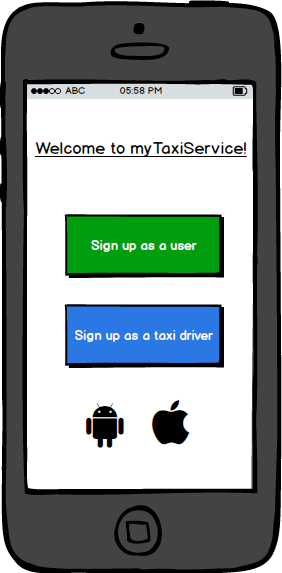
\includegraphics[width=5cm]{./Mockups/SignUp.png}
        \caption{Sign up form}
    \end{minipage}
    \ \hspace{2mm} \hspace{3mm} \
    \begin{minipage}[b]{6cm}
        \centering
        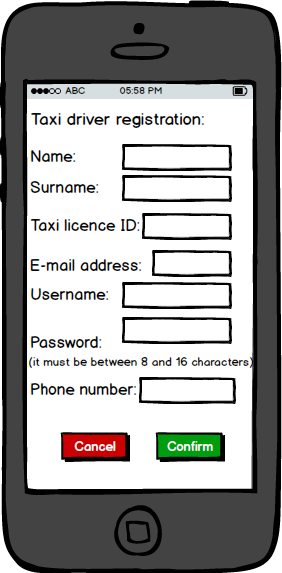
\includegraphics[width=5cm]{./Mockups/TaxiRegistration.png}
        \caption{Taxi registration form}
    \end{minipage}
\end{figure}

\begin{figure}[H]
        \centering
        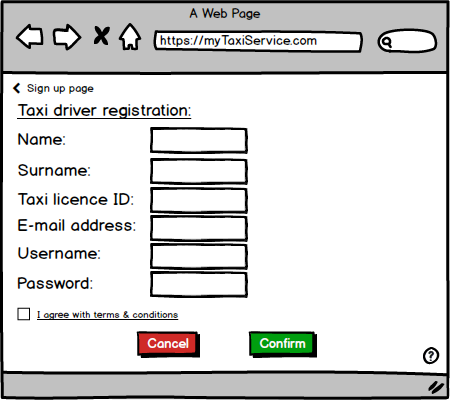
\includegraphics[width=\textwidth]{./Mockups/RegistrationWeb.png}
        \caption{User registration form of the web application}
\end{figure}

